\documentclass[border=10pt]{standalone}
\usepackage{xcolor}
\usepackage{pgfplots}
\usepackage{tikz}
\begin{document}
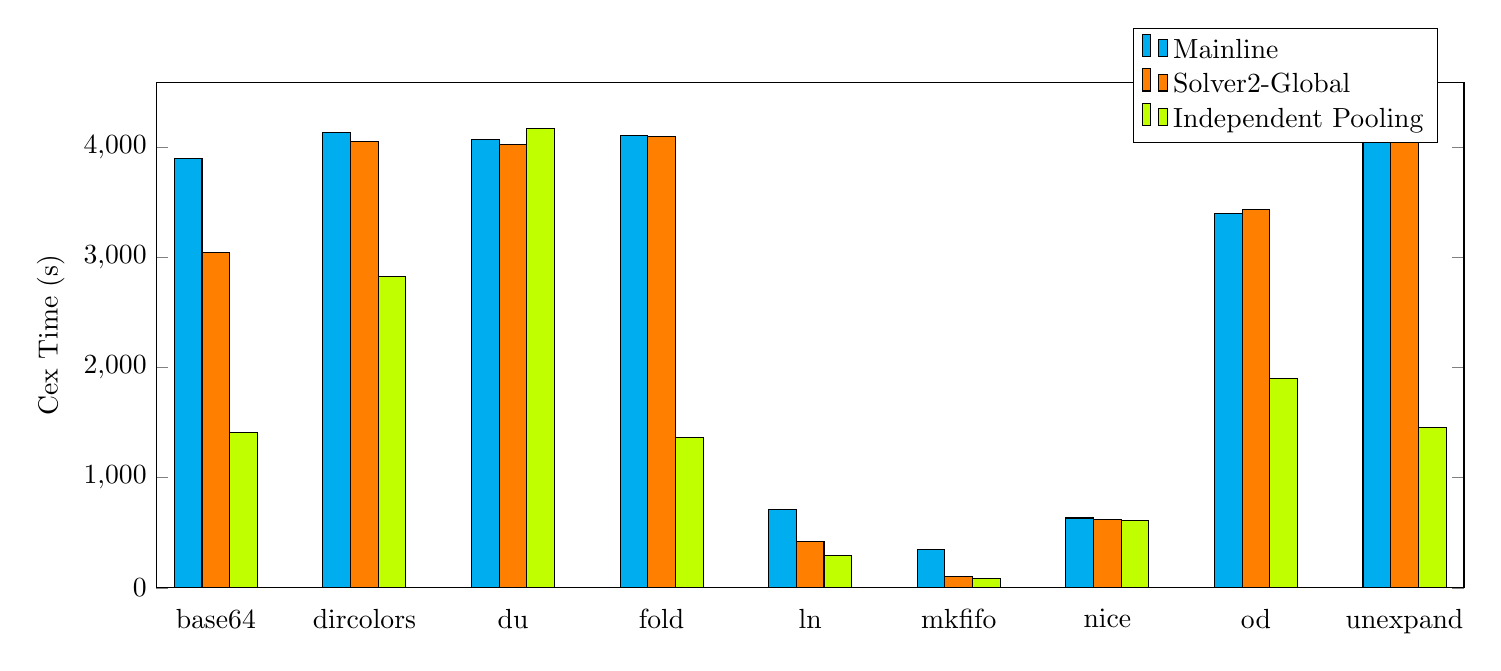
\begin{tikzpicture}
    \begin{axis}[
        width  = 1.5 * \textwidth,
        height = 8cm,
        major x tick style = transparent,
        % tickwidth=10,
        ybar=0,
        bar width=10pt,
        % ymajorgrids = true,
        ylabel = {Cex Time (s)},
        symbolic x coords={base64,dircolors,du,fold,ln,mkfifo,nice,od,unexpand},
        xtick = data,
        scaled y ticks = false,
        enlarge x limits=0.05,
        ymin=0,
        legend cell align=left,
        legend style={
                at={(0.98,0.88)},
                anchor=south east,
                % column sep=1ex
        }
    ]
        \addplot[style={cyan,fill=cyan,mark=none}, draw=black]
	coordinates {(base64,3898.58) (dircolors,4135.06) (du,4070.68) (fold,4103.14) (ln,713.86) (mkfifo,346.26) (nice,634.60) (od,3396.01) (unexpand,4119.88)};
\addplot[style={orange,fill=orange,mark=none}, draw=black]
	coordinates {(base64,3041.34) (dircolors,4055.87) (du,4024.60) (fold,4097.10) (ln,423.86) (mkfifo,104.94) (nice,624.24) (od,3436.30) (unexpand,4121.60)};
\addplot[style={lime,fill=lime,mark=none}, draw=black]
	coordinates {(base64,1410.45) (dircolors,2824.38) (du,4170.54) (fold,1365.08) (ln,297.41) (mkfifo,81.48) (nice,611.20) (od,1897.30) (unexpand,1456.41)};

        \legend{Mainline,Solver2-Global,Independent Pooling}
    \end{axis}
\end{tikzpicture}
\end{document}
